\chapter{Operating System}

\section{Introduction}

An operating system (\textbf{OS}) is the software that manages the computer hardware, creating some logical resources that other software and users can use. It's the logical support which controls and manages the physical components.

\begin{center}
    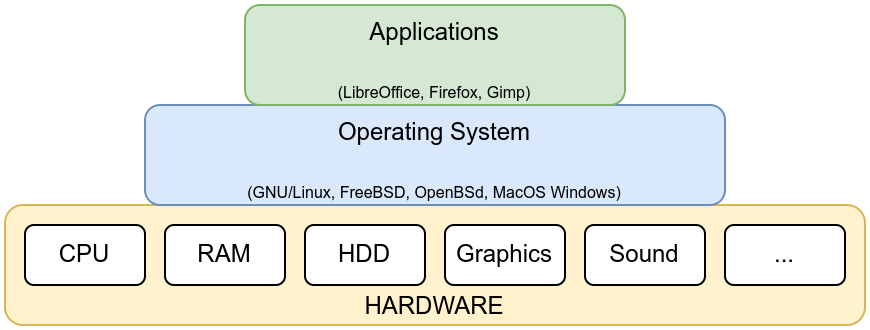
\includegraphics[width=0.9\linewidth]{operating_system.png}
\end{center}

Before the existence of operating systems, the hardware was available directly to the program, so every program must implement the access to the memory, the hard disk, how to read/write files...

\section{Software hierarchy}
The computer runs software, and this software can be classified:

\begin{itemize}
    \item \textbf{System's software}: Controls and manages the hardware of the computer. In this group: \textbf{operating systems}, \textbf{drivers} and \textbf{firmwares}.

    \item \textbf{Service programs}: Those are the networking services, system's services, and some services that the operating system uses. For example: networking management tools, disk partitioners, process manager ...

    \item \textbf{Utility programs}: The software that the end users use in order to do some basic stuff. Word processors, music utilities, games, ...
\end{itemize}


\section{History of operating systems}
Let's see a brief history of operating systems.

\subsection{No operating systems (0-generation)}
The first computers were mainframes (big computers used by organizations), which didn't have any form of operating system.

The user which wanted to use the computer had to  schedule a period of time, because those computers hadn't got time sharing, only one program could run in each time.

First programs were coded in \textbf{machine code}, which is represented with '0' and '1', also called \textbf{binary code}.

Those programs had full access to the hardware, and because of that, every program had to implement access to those resources.

This period started with the digital computers until the late 1950s.

\begin{center}
    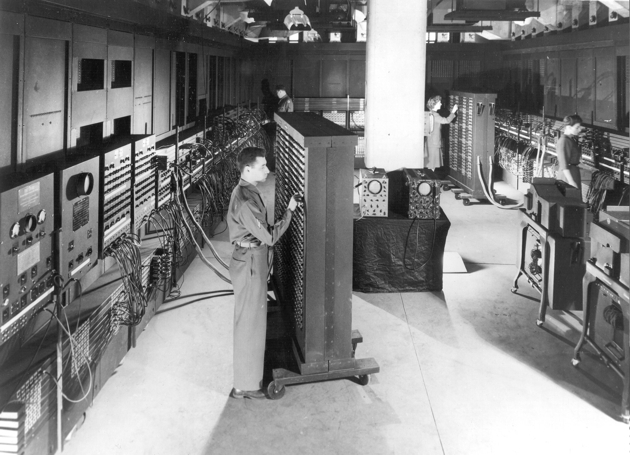
\includegraphics[width=0.6\linewidth]{ENIAC.jpg}
    \vspace{-10pt}\captionof{figure}{\href{https://en.wikipedia.org/wiki/ENIAC}{ENIAC computer. Source: Wikipedia}}\vspace{-13pt}
\end{center}


\subsection{Batch processing (1st generation)}
The computers became faster, and in order to no waste time, the \textit{\textbf{monitors}} were developed (the forerunners of operating systems). Those \textit{monitors} could process a series, or “batch”, of programs, often from magnetic tape.

\begin{center}
    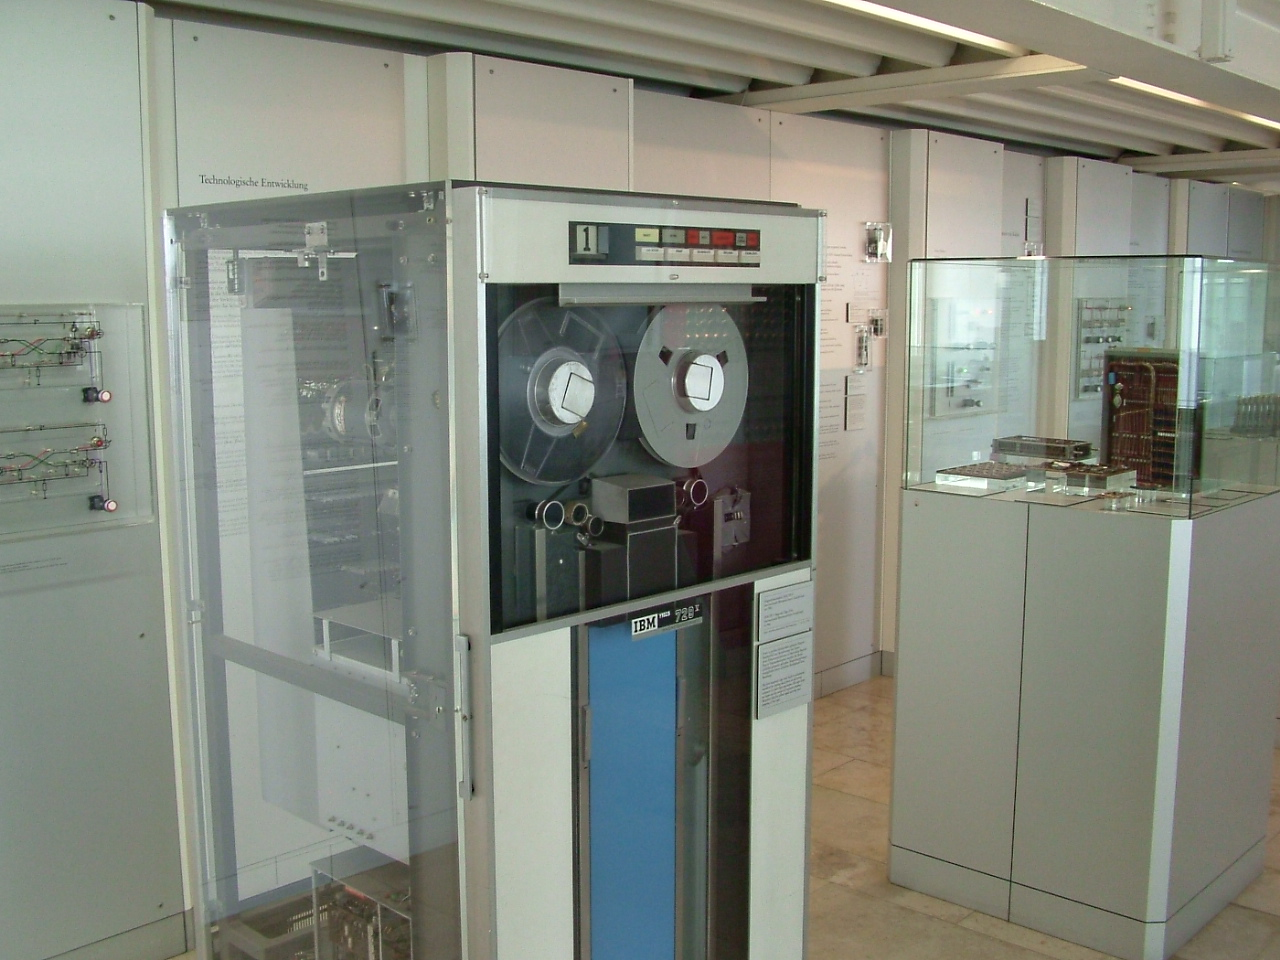
\includegraphics[width=0.6\linewidth]{tape.jpg}
    \vspace{-10pt}\captionof{figure}{\href{https://en.wikipedia.org/wiki/Magnetic-tape_data_storage}{Magnetic tape from IBM. Source: Wikipedia}}\vspace{-13pt}
\end{center}

The monitor would be loaded into the computer and run the first job of the batch. At the end of the job it would regain control and load and run the next until the batch was complete. The \textbf{output} of the batch would be written to magnetic tape or printed.


\subsection{Second generation}
In the 1960s, with the introduction ot the \href{https://en.wikipedia.org/wiki/Integrated_circuit}{integrated circuits}, the computers increased in speed, so the operating systems evolved trying to use this speed, using new techniques:

\begin{itemize}
    \item \textbf{Multiprogramming}: In any modern operating system there can be more than one instance of a program loaded in memory at the same time. For example, more than one user could be executing the same program, each user having separate copies of the program loaded into memory

    \item \textbf{Spooling}: Is a specialized form of multi-programming for the purpose of copying data between different devices. Was used to mediate access to punched card readers and punches, magnetic tape drives, and other slow, sequential I/O devices.

    \item \textbf{Buffering}:\textbf{Data buffer} (or just buffer) is a region of a memory used to temporarily store data while it is being moved from one place to another.
\end{itemize}

\subsection{Third generation}
With the evolution of computers, which began to allow the use of several processors, and more complex systems, operating systems evolved along with them.

\begin{itemize}
    \item \textbf{Multitasking}: Is the concurrent execution of multiple processes over a certain period of time. New tasks can interrupt already started ones before they finish, instead of waiting for them to end.

    When the computer has multiple processors, the multitasking is real, because each processor can execute one process at the same time.

    \item \textbf{Virtual memory}:
\end{itemize}


\section{Operating system's functions}
The Operating Systems has some functions that permits the interaction between the applications and the hardware.

\subsection{Process management}
A process is a program in execution. The OS must allocate resources to processes, enable processes to share and exchange information, protect the resources of each process from other processes and enable synchronization among processes.


